\documentclass[12pt]{article}

\usepackage{graphicx}
\graphicspath{ {./} }

\usepackage{float}
\usepackage{placeins}
\usepackage[bookmarks=true]{hyperref}
\usepackage{textcomp}
\usepackage{booktabs}
\usepackage{verbatim}
\usepackage{underscore}
\usepackage{listings}
\usepackage{lstautogobble}

\hypersetup{pdftitle={SafeStreets DD},
	pdfauthor={Andrea Furlan, Cosimo Russo, Giorgio Ughini},        
	pdfsubject={DD},
	colorlinks=true,
	linkcolor=blue,
	citecolor=blue,
	filecolor=black,
	urlcolor=[rgb]{0.59, 0, 0.78}
}
\lstset{
	string=[s]{"}{"},
	stringstyle=\color{blue},
	comment=[l]{:},
	commentstyle=\color{black},
	autogobble=true
}

\newcommand{\defaultFigure}[3][1]{
	\begin{figure}[h!]
		\makebox[\textwidth]{\includegraphics[width=#1\textwidth]{images/#2}}
		\caption{#3}
	\end{figure}
	\FloatBarrier
}

\begin{document}
	\begin{titlepage}
		\newcommand{\HRule}{\rule{\linewidth}{0.7mm}}
		\center
		
\includegraphics[width=\textwidth]{PolimiLogo.png}\\[1cm]
		
		\textsc{\LARGE Design Document}\\[1cm]
		\textsc{\large Software Engineering II Project - A.Y. 2019-2020}\\[1cm]
		\HRule \\[0.4cm]
		{ \huge \bfseries SafeStreets}\\[0.15cm]
		\HRule \\[1.5cm]
		{\large Authors  \hfill ID Numbers}\\[0.4cm]
		{\large Andrea \textsc{Furlan}  \hfill 944774}\\[0.2cm]
		{\large Cosimo \textsc{Russo}  \hfill 945891}\\[0.2cm]
		{\large Giorgio \textsc{Ughini} \hfill 944710}\\[2cm]
		{\large \today  \hfill Version 1.0}
		\vfill
	\end{titlepage}
\clearpage

{\hypersetup{hidelinks}\tableofcontents}
\clearpage
\setlength{\parskip}{1em}
\section{Introduction}
\subsection{Purpose}
The main purpose of SafeStreets is to create a software that provides users the possibility to notify	
authorities	when parking violations occur providing some useful features such as finding the most unsafe areas around them and proposing suggestions to the municipality. In addition, SafeStreets will enable the Local Police to generate traffic tickets from it and to cross all the information it owns with the data of the accidents happened.\\
Specifically, we want to realize a product which is able to:
\begin{itemize}
	
	\item Retrieve pictures uploaded by users of parking violations with possible attached information such as license plate position in the image, type of violation and GPS meta-data.
	
	\item Automatically complete the data of a reported violation running a recognition algorithm able to read license plate text.
	
	\item Highlight to users the areas with the highest frequency of violations and information about vehicles that commit most violations.
	
	\item Automatically identify	potentially unsafe	areas crossing SafeStreets' information with accident datas from the Local Police, possibly	suggesting	possible	interventions.
	
	\item Send violations data to the Local Police to automatically create new traffic tickets if it can be proved that the	chain	of	custody	of	the	information	coming	from	the	users	is	never	broken.
	
	\item Generate statistics related to ticket emissions to inform users about how effective SafeStreets is.
	
\end{itemize}

On the other hand, the purpose of this paper is to define in a detailed way all the functions and requirements of the application.\\ In doing this, we start focusing on a brief overview to characterize the product with relevance to its interaction with the world, then we will proceed deeply in analysing which functions are relevant and should be provided, and which requirements are needed to the stakeholders. 


\subsection{Scope}
As our software needs to be compliant with different laws and as it needs to interact with the Local Police, initially, SafeStreets will have a restricted geographic domain coincident with the Italian
city of Milan. \\
Indeed, in order to provide the most complete service, SafeStreets will require the access the Local Police web application to be able to process traffic tickets. \\
It goes without saying that to organize this kind of service in the most effective way we must experiment first this activity in a internationally-visible city, then applying that to anyone who will demand.
\clearpage

\subsection{Definition and Acronyms}
\subsubsection{Definitions}
\begin{itemize}
	\item \textit{Data Mining}: The process of discovering patterns in large data sets involving methods at the intersection of machine learning, statistics, and database systems.
	\item \textit{Computer Vision}: The Computer Vision includes methods for acquiring, processing, analyzing and understanding digital images, to extract high-dimensional data from the real world.
	\item \textit{Report}: The data that a user has provided to the authorities that witness a violation by a vehicles.
	\item \textit{Ticket}: Notice issued by a law enforcement official to a motorist or other road user, indicating that the user has violated traffic laws.
	\item \textit{Violation}: The general infraction that a vehicle has done and that has been reported by a SafeStreets user.
	\item \textit{Guest}: This actor plays the role of a person who is not registered and thus logged in.
	\item \textit{User}: This actor refers to the condition of a normal person (not an officer) already signed up.
	\item \textit{Officer} or \textit{Authority}: This actor represents a public officer that interacts with SafeStreets in some ways.
	\item \textit{Customer}: either a Guest or an Authority
\end{itemize}

\subsubsection{Acronyms}
\begin{itemize}
	\item \textbf{AI}:\@ Artificial Intelligence
	\item \textbf{API}:\@ Application Programming Interface
	\item \textbf{CMS}:\@ Content Management System
	\item \textbf{IEEE}:\@ Institute of Electrical and Electronic Engineers
	\item \textbf{GPS}:\@ Global Positioning System
	\item \textbf{OCR}:\@ Optical Character Recognition
	\item \textbf{TLS}:\@ Transport Layer Security
	\item \textbf{UML}:\@ Unified Modeling language
\end{itemize}

\subsection{Revision}

\subsection{References}
\begin{itemize}
	
	\item The 2019-2020 Software Engineering 2 Project Assignment document
	\item The IEEE Standard for DD
	\item The RASD of SafeStreets
	
\end{itemize}

\subsection{Document Structure}
This document is divided in four parts:
\begin{itemize}
	\item \textbf{Introduction}: a description about the goals of SafeStreets and the context in which it will be implemented is provided. A subsection dedicated to the understaing of some acronyms and definitions is also present. 
	
	\item \textbf{Overall Description}: gives an overall description of SafeStreets, focusing on the domain assumptions and the constraints of the application. This section also aims to provide a context to the whole project and to show its integration with the real world. It also shows the possible interactions between the world and the users of SafeStreets. 
	
	\item \textbf{Specific Requirements}: the software requirements, explained in a sufficiently detailed manner to design a system that satisfies them, and the testers to test said requirements are provided.
		
		A detailed description of the possible interactions that can occur between the world and the system is also present, followed by a series of simulations and previews about the interactions mentioned above.
	
	\item \textbf{Formal Analysis using Alloy}: the requirements are expressed through the Alloy model, which, being it is a declarative specification language, makes it possible to define the functions, the constraints and the interactions of SafeStreets.
\end{itemize}
In the last part of the document a short note about the softwares used and the effort spent in producing this RASD by its authors is shown.
\clearpage

\section{Architectural Design}
\input{subsections/section2/architecturalDesign}
\subsection{Overview}
The logical division of the application consists of 3 layers: presentation, application and data.

\subsubsection{Presentation layer}
the presentation layer consists of a mobile application for the users and a website for the officers.
The application will be available from the major app stores while the website will be distributed through a web server.
It is important to note that both the application and the website will only provide the user interface and will retrieve data from the application layer.

\subsubsection{Application layer}
This layer will employ a microservices architecture.
Each microservice will handle a single functionality of the application in an atomic and stateless manner.
Also, each service will expose a REST interface accessible over HTTPS to be able to handle requests from the clients, the police systems and other microservices.

Microservices will be deployed in containers that will be able to efficiently scale based on the load on the single service, thus ensuring maximum scalability and elasticity and never wasting resources.
Since microservices are stateless by definition, redundancy can be easily implemented. This is a key point toward the availability requirement.

This architecture opens the possibility for some services to be bought instead of being implemented from scratch. For example the login/registration service will use the \href{https://cloud.ibm.com/catalog/services/app-id#about}{App ID} service from IBM instead of a homemade solution.

The main services are:
\begin{itemize}
    \item \textbf{Login and registration}
    \item \textbf{Violations and Tickets management}
    \item \textbf{Statistics}
    \item \textbf{Metadata acquisition in images} - exploits computer vision to extract info from pictures, like the car color and model
    \item \textbf{Tickets checking} - exploits computer vision to automatic check tickets, using information from different sources
    \item \textbf{Unsafe positions calibration} - uses an AI to adjust the unsafe positions recommendations based on those that were previously accepted/rejected
\end{itemize}

\subsubsection{Data layer}
Each microservice will have its own storage engine that cannot be directly contacted by other services. In particular:
\begin{itemize}
    \item the \textbf{login and registration} and the \textbf{violation and tickets management} services will have a relational database. These services will probably be the most used and will therefore exploit database distribution techniques.
    \item the \textbf{statistics} service will use a data warehouse to perform complex queries and a non-relational database engine to cache the most used results
    \item both the computer vision services will retrieve data from the violation service and use the storage system of the provider of these services
    \item the unsafe position calibration service will retrieve data from the violation service and the police service and store them on its relational database, other data structure specific for the AI implementation will depend on the external provider of this service
\end{itemize}

All storage systems must have replicas and scheduled backups in order to avoid data loss.
\subsection{High-Level components: general architecture identification}\label{higharch}
The logical division of the application consists of 3 layers that will be shown here: presentation, application and data.
\\Here we provide for each tier the definition, choice reasons and used technology:
\subsubsection{Presentation layer}\label{presentationlayer}
the presentation layer consists of a mobile application for the users and a website for the officers.
The application will be available from the major app stores while the website will be distributed through a web server.
It is important to note that both the application and the website will only provide the user interface and will retrieve data from the application layer.

\subsubsection{Application layer}\label{applicationlayer}
This layer will employ a microservices architecture.
Each microservice will handle a single functionality of the application in an atomic and stateless manner.
Also, each service will expose a REST interface accessible over HTTPS to be able to handle requests from the clients, the police systems and other microservices.

Microservices will be deployed in containers that will be able to efficiently scale based on the load on the single service, thus ensuring maximum scalability and elasticity and never wasting resources.
Since microservices are stateless by definition, redundancy can be easily implemented. This is a key point toward the availability requirement.

This architecture opens the possibility for some services to be bought instead of being implemented from scratch. For example the login/registration service will use the \hyperlink{appidsafestreets}{App ID} service from IBM instead of a homemade solution.

The main services are:
\begin{itemize}
	\item \textbf{Users Management} - Login and registration
	\item \textbf{Violations and Tickets management}
	\item \textbf{Tickets Hashing system} - Allows the police to check for the integrity of a ticket by comparing an hash
	\item \textbf{Statistics}
	\item \textbf{Tickets checking} - Exploits computer vision and data mining to automatically check tickets, using information from different sources. Tickets that are suspected to be invalid are then sent to the local police for a double check.
	\item \textbf{Unsafe positions} - Uses an AI to extract unsafe positions from violations and accidents and to provide a possible solution to it. Such solutions are then available for the local police.
	\item \textbf{Computer Vision} - Extract info from pictures, like the car color and model
	\item \textbf{Data Mining} - Extracts patterns from huge amounts of data useful for other services
\end{itemize}

\subsubsection{Data layer}\label{datalayer}
Each microservice will have its own storage engine that cannot be directly contacted by other services. Pay-per-use services, such as \textit{Users management}, have their internal storage system that is abstracted,
for the services that need a storage system it will be hosted in the cloud and managed by IBM, billed per GB used. This system is the best possible abstraction for scalability.

All storage systems are guaranteed to have replicas and scheduled backups in order to avoid data loss.
\subsection{Component View}\label{componentview}
\subsubsection{Database overview}
\subsubsection{Database}
Each microservice will have its own data storage system. All the systems must obey to the laws regarding data protection (like GDPR), which means that:
\begin{itemize}
\item Sensible data such as passwords and personal information must be encrypted properly before being stored in the selected microservice.
\item Users must be granted access only upon provision of correct and valid credentials
\end{itemize}

Here we include all the E-R diagrams for all microservices

%Mettiamo qui il diagramma ER del db
\subsubsection{Microservices}\label{microservices}
In this subsection it is explained which microservices will be custom and which one will be used as pay-per-use. 
\\All microservices will be stored in the Cloud offered by IBM and every microservice is picked from the IBM Cloud Platform.
\\For services that are used with the pay-as-you-go mechanism it is briefly explained how they work and some diagrams are included to better understand the concept.
\begin{itemize}
	\item \textbf{Login - \href{https://cloud.ibm.com/catalog/services/app-id}{IBM App ID}}: This microservice is about User Authentication and Management, and provides a log-in framework. App ID will be used to add authentication to our web and mobile apps securing our Cloud-native applications and services on IBM Cloud. By requiring users to sign in to our app, we will be able to store user data such as app preferences or information from public social profile to recognize user that reports violations and customize each user's experience within the app.
	\\When a user is successfully authenticated, the application receives tokens from App ID. The service uses three main types of tokens to complete the authentication process: Access Token, Identity Token and Refresh Token.
	\begin{figure}[h!]
		\makebox[\textwidth]{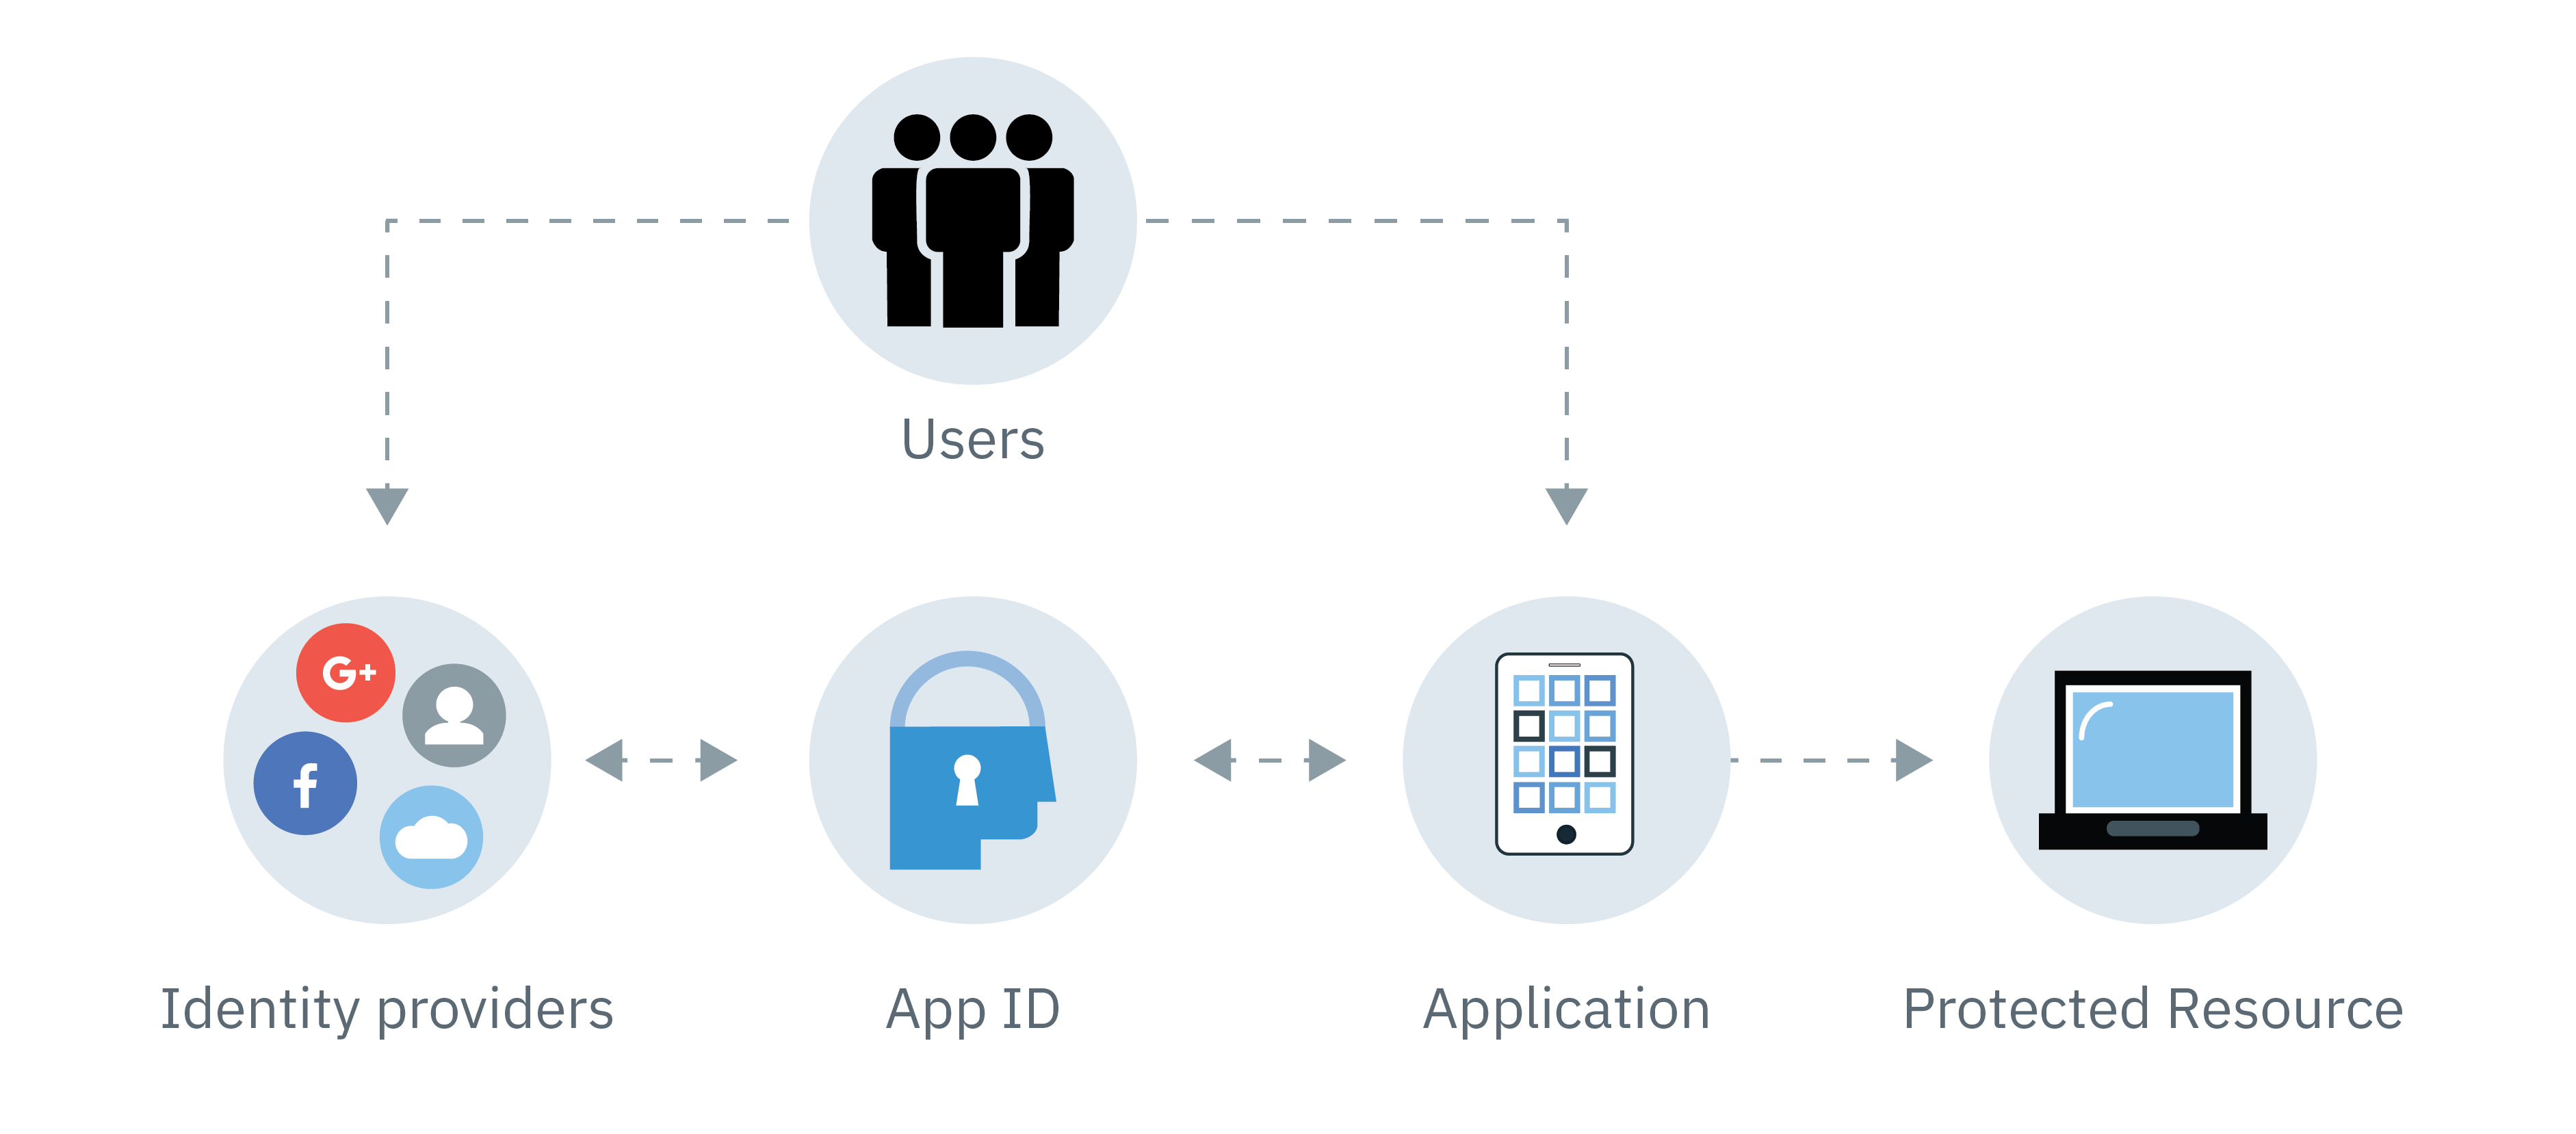
\includegraphics[width=1.15\textwidth]{/images/microservices/appidarchitecture.png}}
		\caption{IBM App ID working diagram.}
	\end{figure}
	\FloatBarrier

	\item \textbf{Computer Vision - \href{https://cloud.ibm.com/catalog/services/visual-recognition}{IBM Watson Visual Recognition}}: This service uses deep learning algorithms to analyze images for scenes, objects, and other content. In our scenario it will be used for certifying automatic tickets and to extract various information from violation's pictures.
	\\Its usage is simple as making an HTTP request to its POST API sending the image then wait for it to finish his work. The response that it returns includes keywords that provide information about the content along with an estimate probability of them being identified.
	\\In addition, IBM Watson Visual Recognition supports high availability with no single point of failure. Recovering from potential disasters that affect an entire IBM location requires planning and preparation but can always be done saving all of our custom training model.
	\begin{figure}[h!]
		\makebox[\textwidth]{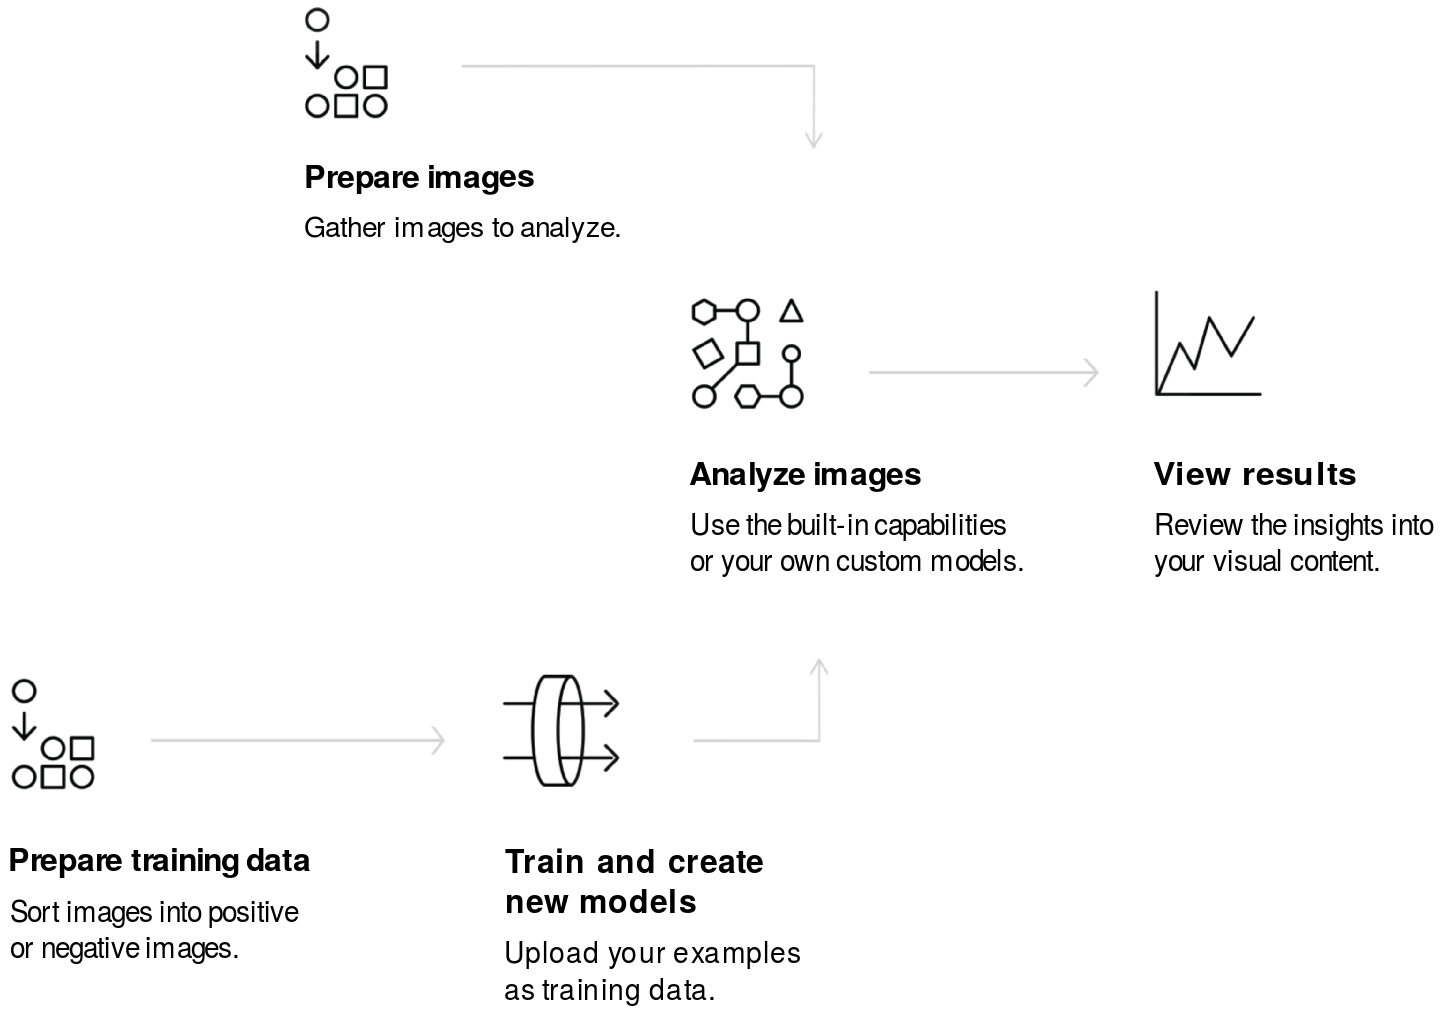
\includegraphics[width=1.15\textwidth]{/images/microservices/visualrecognition.png}}
		\caption{IBM Watson Visual Recognition working diagram.}
	\end{figure}
	\FloatBarrier
	
	\item \textbf{Data Mining - \href{https://cloud.ibm.com/catalog/services/discovery}{IBM Watson Discovery}}: IBM Watson Discovery makes it possible to rapidly build cognitive, cloud-based exploration applications that unlock insights hidden in unstructured data. 
	\\This microservice is particularly useful when, at a given time everyday, SafeStreets crosses data coming from the municipality with its own data to extract potential suggestions.
	\\With Discovery, it only takes a few steps to prepare our unstructured data coming from different sources and to create a query that will pinpoint the information SafeStreets needs. Discovery automatically uses data analysis combined with cognitive intuition to take the unstructured data and enriches it to discover hidden information.
	\begin{figure}[h!]
		\makebox[\textwidth]{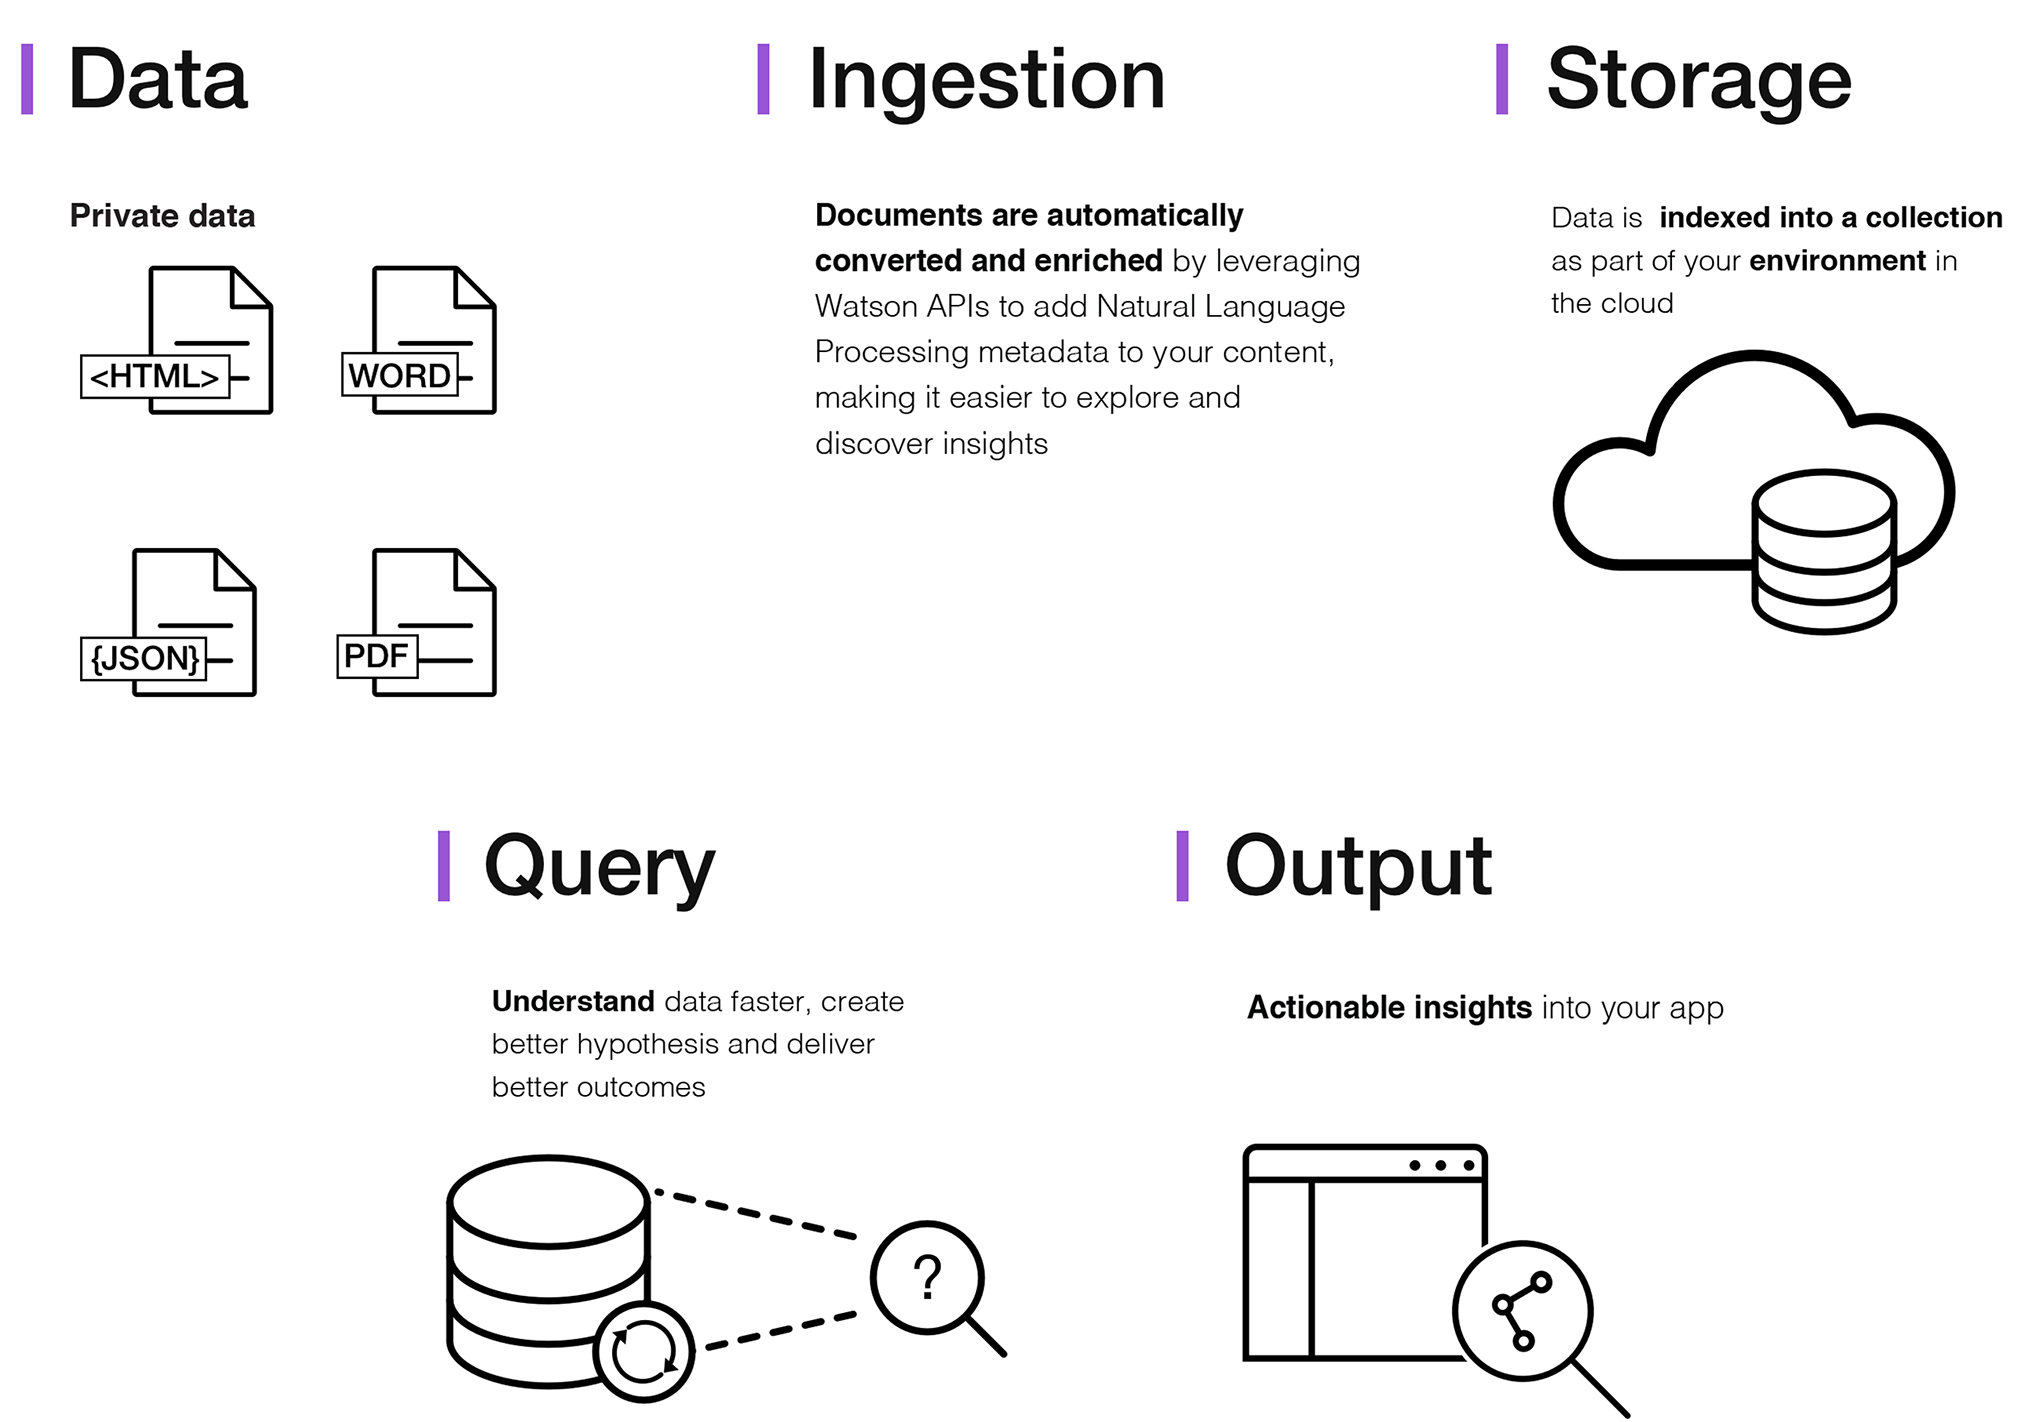
\includegraphics[width=1.25\textwidth]{/images/microservices/discoveryflow.png}}
		\caption{Complete architecture of our Discovery solution.}
	\end{figure}
	\FloatBarrier
	
	\item \textbf{Image Storage - \href{https://cloud.ibm.com/catalog/services/cloud-object-storage}{IBM Cloud Object Storage}}: When a user sends one or more pictures in a report along with various information on the violation he's reporting, these files must be obviously stored somewhere. In our case, to ensure  resiliency and the other proprieties expressed in the RASD, we opted for storing these image in the IBM Cloud. Indeed, information stored in the IBM Cloud Object Storage is encrypted and dispersed across multiple geographic locations, and accessed over HTTP using a modern RESTful API.
	In addition, IBM Cloud Object Storage allows SafeStreets to separate metadata from the image, but store them as objects in the same storage. That means that for every image, SafeStreets can associate it with highly unstructured data, different for each image. 
	\\For example when someone reports a violation, the related images are instantaneously saved in the Storage, along with their metadata. Then, when the Computer Vision algorithm takes place on them, the metadata of such images will be updated with a PUT request with the information that it will extract (such as the presence of no-parking signs).
	\\Last but not least, the IBM Cloud Object Storage can be easily associated with IBM Discovery as an external source for training.
	\begin{figure}[h!]
		\makebox[\textwidth]{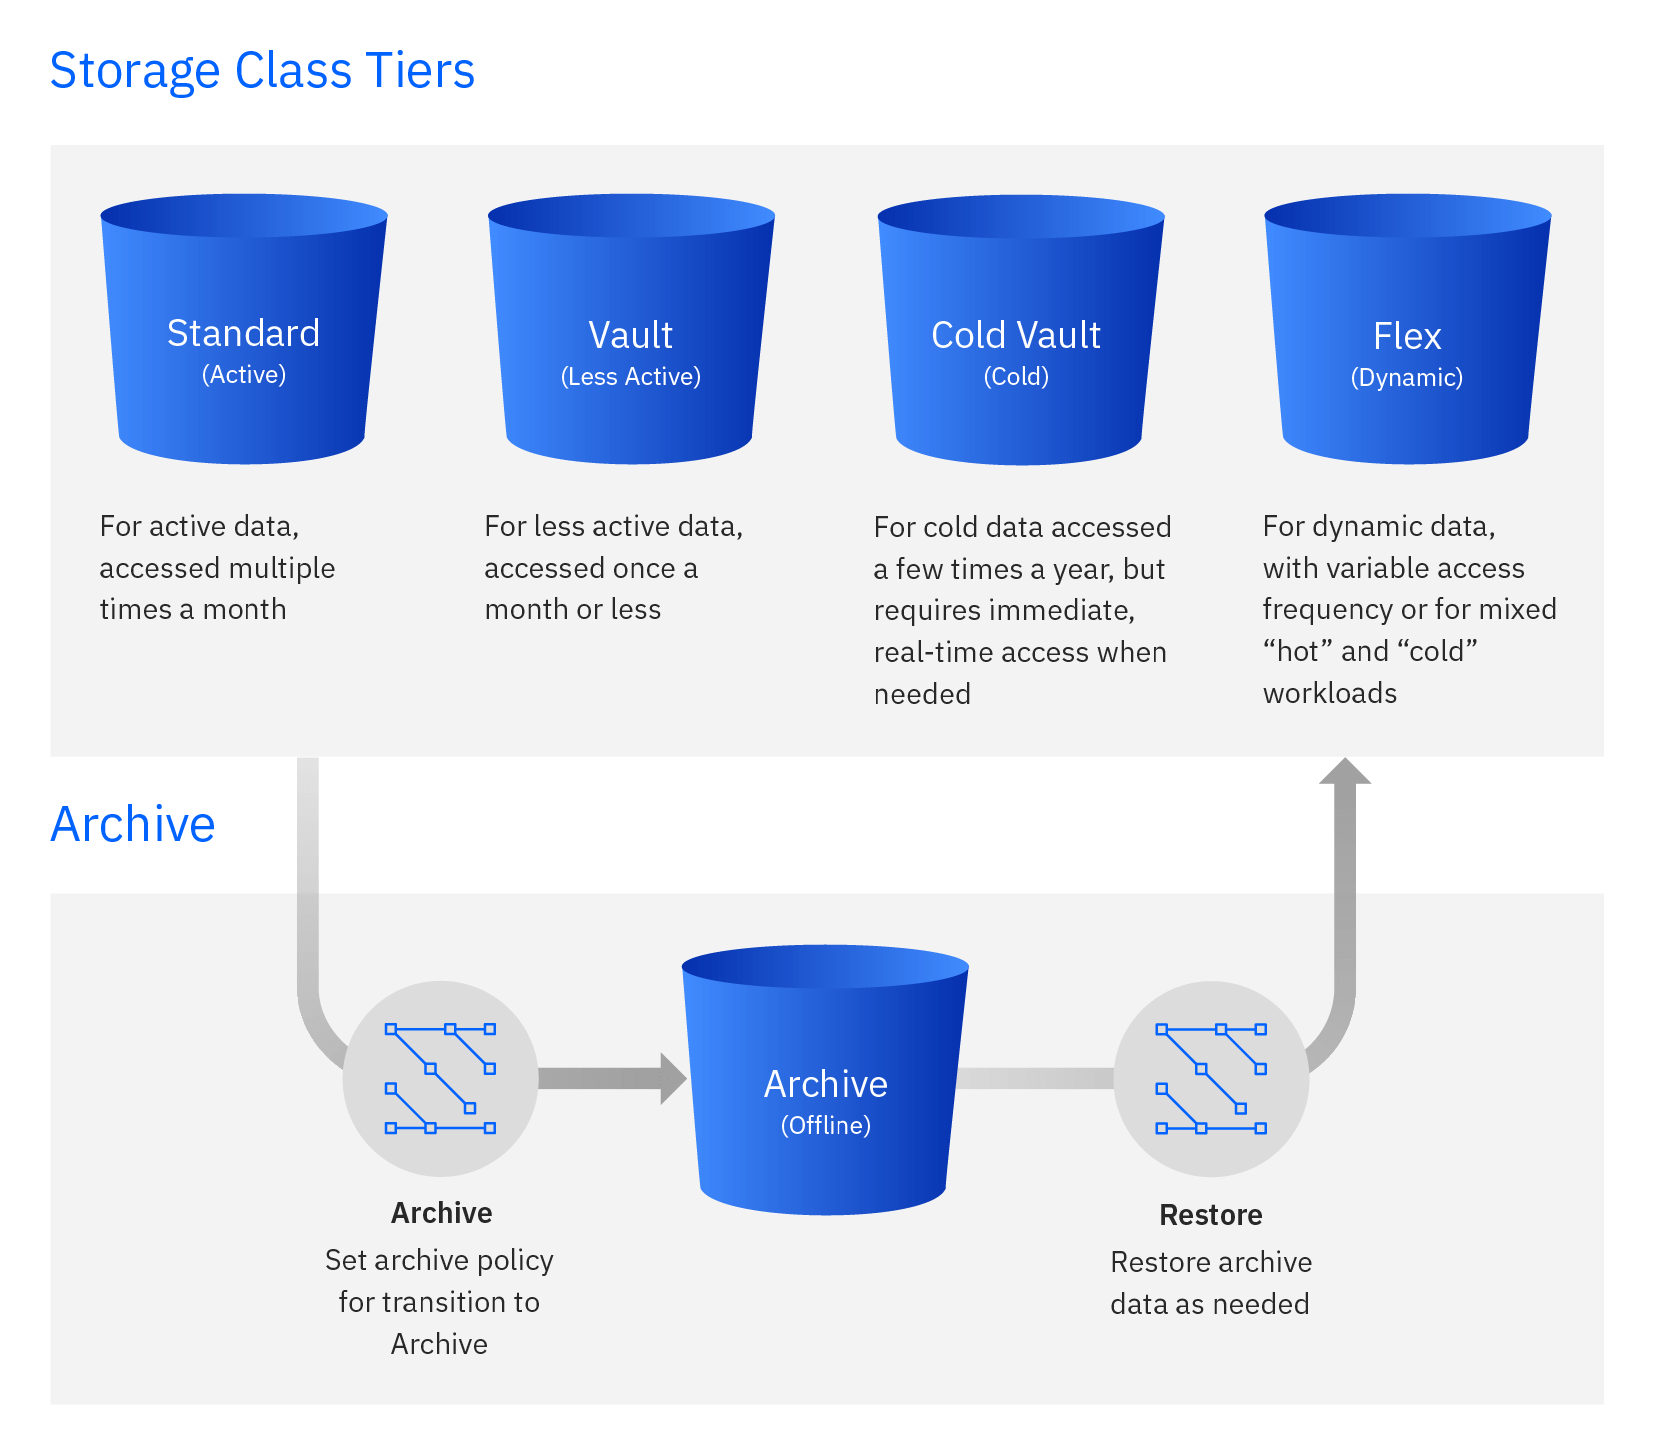
\includegraphics[width=0.95\textwidth]{/images/microservices/policybasedarchive.png}}
		\caption{IBM automatically tier data to the lowest-cost archive.}
	\end{figure}
	\FloatBarrier
	
	\item \textbf{NoSQL Database - \href{https://cloud.ibm.com/catalog/services/cloudant}{IBM Cloudant}}: IBM Cloudant is a distributed database that is optimized for handling heavy workloads that are typical of large, fast-growing web and mobile apps. Available as an SLA-backed, fully managed IBM Cloud service, Cloudant elastically scales throughput and storage independently.
	\\SafeStreets will use Cloudant every time a NoSQL Database is required, for example to manage the highly unstructured data in the Suggestion DB.
	Moreover, Cloudant is ISO27001, SOC 2.2 compliant and HIPAA ready. All data is encrypted over the wire and at rest. The service integrates with IBM Authentication and Management (IBM App ID) for granular access control at the API level.
	\\Using this service, SafeStreets will not need any server (Cloudant is serverless) and its data will be automatically replicated closer to all the places it needs to be, for uninterrupted data access.
	\begin{figure}[h!]
		\makebox[\textwidth]{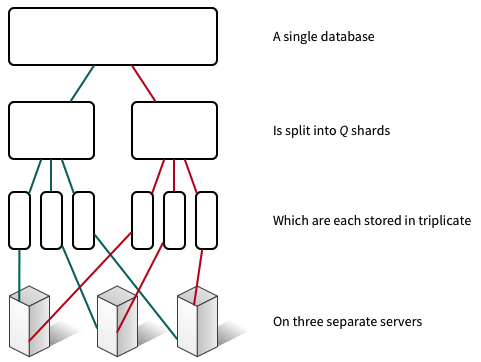
\includegraphics[width=0.9\textwidth]{/images/microservices/shardingdatabase.png}}
		\caption{How is data stored in IBM Cloudant}
	\end{figure}
	\FloatBarrier
	All Q shards together contain the data within database. Each shard is stored in three separate copies. Each shard copy is called a shard replica. Each shard replica is stored on a different server. The servers are available within a single location data center. The collection of servers in a data center is called a cluster.
	\begin{figure}[h!]
		\makebox[\textwidth]{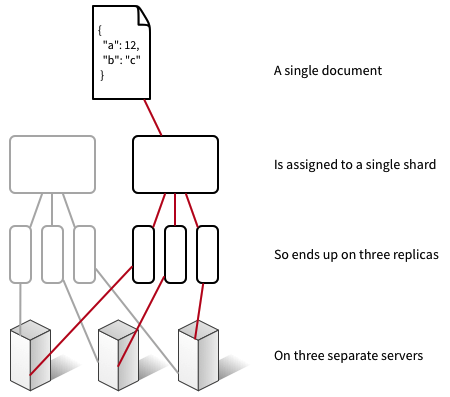
\includegraphics[width=0.9\textwidth]{/images/microservices/shardingdocument.png}}
		\caption{How is data stored in IBM Cloudant}
	\end{figure}
	\FloatBarrier
	
	\item \textbf{Relational Database - \href{https://cloud.ibm.com/catalog/services/databases-for-postgresql}{IBM Cloud Databases for PostgreSQL}}: A relational DBMS was chosen for all the Databases that contains structured data and on which many queries will be done (Violation, Statistics). Postgres was chosen over all database because it is a powerful, open source object-relational database with JSON support, that gives the best of both the SQL and NoSQL worlds. The advantages in using an IBM Cloud Service to deploy such service relies on the fact that this service allows us to scale disk and RAM independently to best fit SafeStreets application requirements.
	\\IBM Cloud Databases provide out-of-the-box integration with IBM Identity and Access Management that integrates completely into the SafeStreets architecture. 
	\begin{figure}[h!]
		\makebox[\textwidth]{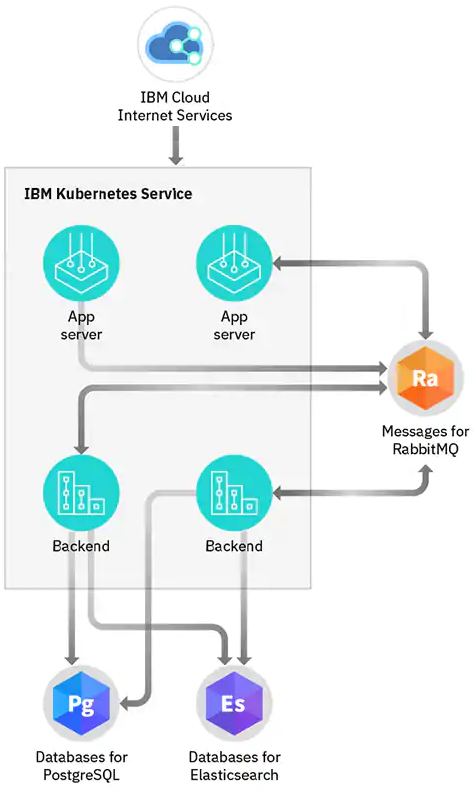
\includegraphics[width=0.7\textwidth]{/images/microservices/postgres.png}}
		\caption{Scalable SafeStreets architecture to handle millions of users.}
	\end{figure}
	\FloatBarrier
	
\end{itemize}
\clearpage
\subsubsection{Database components}\label{databasecomponent}
Having provided a detailed description of the types of DBMS services we will use to store data, we can proceed to explain in detail how they will be organized.
\begin{itemize}
	\item \textbf{Violations Database - \href{https://cloud.ibm.com/catalog/services/databases-for-postgresql}{Relational PostgreSQL Cloud Database}}: The Violations Database is the most important Database of the whole SafeStreets architecture. Inside it, it will be found all the reported infraction along with a link to the Object Storage where the pictures of each violation are. For this reason, there will be two read replicas of the PostgreSQL Violations DB to offload traffic from our leader database. 
	\\As IBM Cloud Databases allows to scale disk and RAM to best fit the application requirements, it is not needed to state how much memory and disk space the database must have, it just needs to be deployed. After the deployment, all the microservice that needs to access data inside this database, will be given a connection string that allows read or read/write access depending on which service is.
	%TODO: Add schema model
	\begin{comment}
	\begin{figure}[h!]
		\makebox[\textwidth]{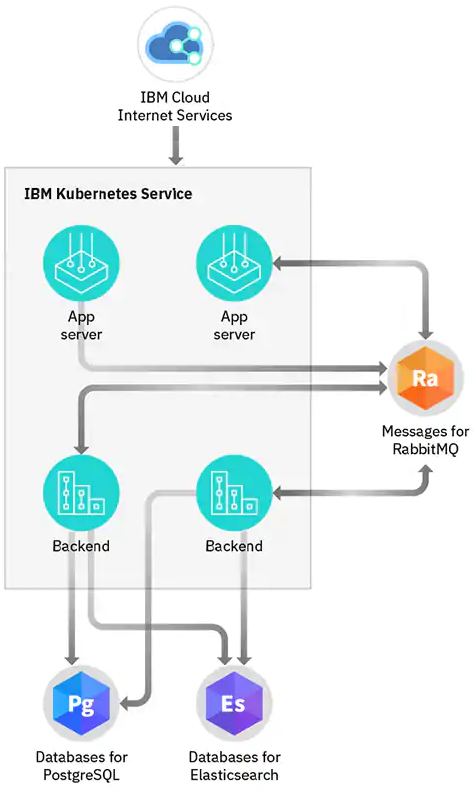
\includegraphics[width=0.7\textwidth]{/images/microservices/postgres.png}}
		\caption{Scalable SafeStreets architecture to handle millions of users.}
	\end{figure}
	\FloatBarrier
	\end{comment}
	
	\item \textbf{Suggestion Database - \href{https://cloud.ibm.com/catalog/services/cloudant}{IBM Cloudant}}: This database represents the core heart of the memory that stores all the data that comes from the AI and Data Mining algorithms.
	\\Our system will be configured such as when it detects that is in a low-traffic moment, if it's in a time shift to be configured (late night) then it will start to mine the data of the past day to find possible suggestion to unsafe areas. When it finishes, the newly created suggestion will be stored in this database.
	\\As every suggestion comes from an Artificial Intelligence agents, it would be substantially different in structure from each other, and so it needs to be stored in a NoSQL database such as Cloudant. Figure \ref{fig:jsondoc} shows some possible documents that can be stored inside this database.
	\\This instance of Cloudant will be configured to accept read-only queries only from verified Public Police Officers.
	\begin{figure}[h!]
		\begin{lstlisting}
		{
		  "infraction": "Illegal parking",
		  "timeShift": 2019
		  "area": "Via Bassini",
		  "reportsCount": 1821,
		  "ticketsGiven": 1437,
		  "unsafeArea": yes,
		  "incidents": 24,
		  "causedDeath": false,
		  "suggestions": [
			{
			  "suggestion": "Avoid illegal parking"
			  "actions":
			    [ 
				  {
				    "action": "Warn drivers with a flyer",
				    "score": 60.2
				  },
				  {
				    "action": "Make more tickets",
				    "score": 58.7
				  }
			    ]
			},
			{
			  "suggestion": "Make ZTL from 5PM"
			  "actions":
			    [ 
			      {
			        "action": "Install cameras",
			        "score": 80.2
			      }
			    ]
			}
		  ]
		}
		\end{lstlisting}
		\caption{Example of suggestion document.}
		\label{fig:jsondoc}
	\end{figure}
	\FloatBarrier
	
	\item \textbf{Statistics Database - \href{https://cloud.ibm.com/catalog/services/databases-for-postgresql}{Relational PostgreSQL Cloud Database}}: The Statistics Database where all the application usage statistics are. 
	These are not so important data so for what concerns the replication, it will not physically duplicated by us, but we rely on the internal data replication of IBM.
	\\As already stated, IBM Cloud Databases allows to scale disk and RAM to best fit the application requirements, but in this case is defined a maximum number of resources to be allocated because the statistics page is not a SafeStreets core functionality.
	After the deployment, everyone can query this database trough an apposite microservice, but the write access is restricted only to enabled services inside the IBM Cloud VPN.
	%TODO: Add schema model
	\begin{comment}
	\begin{figure}[h!]
	\makebox[\textwidth]{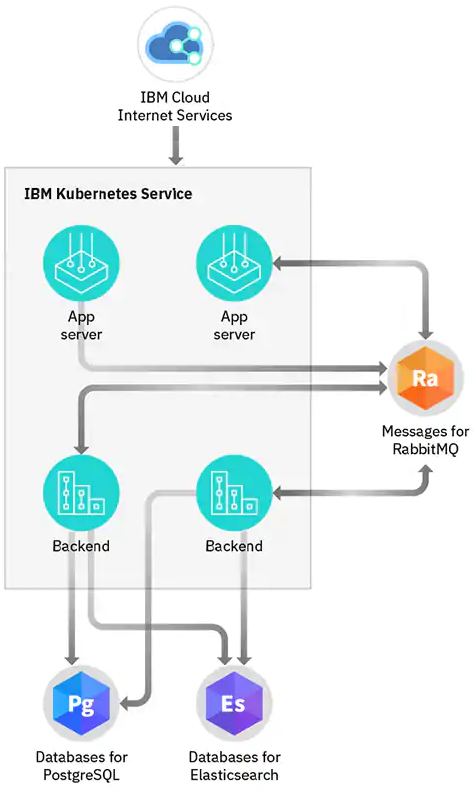
\includegraphics[width=0.7\textwidth]{/images/microservices/postgres.png}}
	\caption{Scalable SafeStreets architecture to handle millions of users.}
	\end{figure}
	\FloatBarrier
	\end{comment}
	
	
\end{itemize}
\subsubsection{High-level component diagram}
This section provides a high level diagram of the architecture of SafeStreet, listing all the microservices and how they are structured in the cloud.

\defaultFigure[1.15]{HighLevelArchitecture.png}{High level architecture}

As show from the figure above, our architecture is composed of several microservices and a web server hosted inside the IBM cloud.

The service inside the box called \textit{first line} are directly accessible for the user, so they will expose an API through a public URL.
Those inside the \textit{support} box provide functions and data to the first line service and will not be exposed outside of the IBM network.

The only purpose of the web server is to serve the static webpages for the CMS system of the local police.
\subsubsection{Low-level component diagram}
In this section each component of the high level components diagram is analysed in more details, explaining
its internal structure.

\defaultFigure[1.15]{LowLevelArchitecture.png}{Low level components diagram}
\begin{itemize}
    \item \textbf{Webserver} - 
    The webserver is containerized in a Docker Apache container and orchestrated by the \hyperlink{kubernetes}{Kubernetes service} for IBM.
    This composition allows to scale the server horizontally by just adding or removing containers with few click based on the load on the server.

    \item \hyperlink{cloudObjectStorage}{\textbf{Cloud Object Storage}}
    All the images will be stored on this component and will be accessible by a public URL. Metadata received from the computer vision service will be store here as metadata of the image they belong to.

    \item \textbf{Violations and Tickets}
    Receives violations from users and gives access to violations to officers and other microservices. It consists of a proprietary web application that exposes a REST API and is connected to a managed \hyperlink{postgres}{PostgreSQL database}.

    \item \textbf{Tickets hashing system}
    Stores the hash of the violations with automatic ticket option on a database that allows only inserts and reads.
    It provides an API for the \textit{Violations and tickets} service to POST a ticket, of which it will calculate the hash,
    and for the police to send and hash for a ticket that will be compared with the one stored in its database.

    \item \textbf{Statistics}
    A simple Python application that every day, when the load on the system is low, contacts the \textit{Violations and tickets} service to grab the violations for that day and builds new statistics that stores inside its \hyperlink{cloudant}{Cloudant database}.
    It also provides and API for users and officers to query for such statistics.

    \item \textbf{Suggestions}
    Uses the power of the \hyperlink{watson}{computer vision} and \hyperlink{discovery}{data mining} services to identify unsafe areas and to provide
    suggestions on how to fix them. It consists of a Python application that queries data from such services and provides an API for the local police to retrieve the
    suggestions found, which are stored in a relational database.

    \item \textbf{Other services}
    The \hyperlink{watson}{computer vision}, \hyperlink{discovery}{data mining} and \hyperlink{appid}{User management} services are well described in other sections and do not have any components relevant here since they are pay-per-use services.
\end{itemize}

\subsection{Deployment View}\label{deploymentview}
The following diagram explains how the application is deployed. Since most of the physical details are hidden behind the IBM services the diagram is custom but still quite straightforward.

Users connect through a smartphone application, while officers use a website that runs in all major browsers. Both the devices can expolit a cache system allowing them to save bandwidth.

The IBM cloud provides a firewall and DDoS protection system, it is included by default when using IBM services and does not need to be managed.

The web server shows 2 instances of the docker container in the graph, which is the starting point for the application. However, it is almost immediate to add new instances and IBM offers an automatic load balancer service for Kubernetes that works out of the box.

All the services inside the \textit{services} box are able to talk to each other without exposing an URL to the network outside of IBM exploiting IBM connection mechanisms. In particular, those inside the green box \textit{private connection} have a reserved connection that can hide them even from other IBM services. This schema is used to isolate databases, while the Python applications are exposed to other microservices and to the external world by means of an API.

The \textit{App ID} service exposes an API to the outside world, while the \textit{Data Mining} and \textit{Computer Vision} services are only available inside the IBM network.

\defaultFigure[1.2]{DeploymentView.png}{Detailed structure of the deployment}
\subsection{Runtime View}\label{runtimeview}
\subsubsection{Signup/Login}
This diagram shows how the app handles all the unauthorized requests. It works in the same way for all the requests that require authentication and for all the microservices.

When the user contacts the microservices without being logged in, he is redirected to the login/registrazion page, where he sends the login information directly to App ID, which responds with a token. The user can then use this token to identify itself with all the microservices, even if his path started from another one.
\defaultFigure[0.8]{sequenceDiagrams/LoginRegistration.png}{sequence diagram of the login process}

From now on we will suppose that each request that requires authentication already has a token.

\subsubsection{Create Violation}
When a user submits a violation, the request is split into 2 parts: first, the pictures are stored in the Cloud Object Storage and their URLs are collected by the user client, then the text fields, along with the URLs, go directly to the violations microservice.

The pictures are sent to the computer vision service to retrieve metadata, identifying objects in the picture. In parallel, the data regarding the violation (vData) is stored inside the violations database. Once the metadata have been retrieved, the couple (vData, metadata) is sent to both the statistics and the data mining microservices.
\defaultFigure[1.15]{sequenceDiagrams/CreateViolation.png}{sequence diagram of the creation of a violation}
\clearpage
\subsection{Component Interfaces}\label{componentinterfaces}
This sections includes further details on the interfaces between the custom internal components of the system and the IBM micro-services illustrated before. The communications among components should take place only through APIs, some of them need to be custom developed and others are already exposed by the services described in \ref{microservices}.
\\ A list of APIs needed for the application's well being are briefly described in the following list, grouped by functionality that interacts through them:

\textbf{User Data Management:}
\begin{itemize}
	\item \textbf{[POST] changePassword(userId,newPassoword):} Used from the client application to change the password of its user.
	\item \textbf{[POST] banUser(userId):} Used from the officers portal in order to ban a malicious user of the application.
\end{itemize}

\textbf{Violations:}
\begin{itemize}
	\item \textbf{[POST] sendViolation(violation):} Used from the client application when a user wants to send a new ticket violation.
	\item \textbf{[GET] getViolationById(violationId):} Used from the officers portal to get the information of a specific violation.
	\item \textbf{[GET] getViolationsByUser(userId):} Used from the client application to get all the user's violations.
	\item \textbf{[GET]	getViolationsPending():} Used from the officers portal to get all the violation that are yet to be processed.
	\item \textbf{[POST] changeViolationState(violationId,newState):} Used from the officers portal to change the status of a violation just analyzed from PENDING to ACCEPTED/DENIED.
	\item \textbf{[GET] getPositionWithGPS(x-coordinates,y-coordinates):} Used from the client application to get the user's position given their GPS position.
\end{itemize}

\textbf{Data Mining:}
\begin{itemize}
	\item \textbf{[GET] getLicensePlate(images,oldLicensePlates):} Used from the client application to get a license plate from the images provided if found. The API should also accept a set of wrong license plate in case the precedent output of the API call was wrong and the user realized that the license plate given didn't correspond to the actual license plate of the vehicle committing the violation.
\end{itemize}

\textbf{Request for interventions:}
\begin{itemize}
	\item \textbf{[GET] getSuggestions(area):} Used from the officers portal to get the possible suggestions elaborated with the data mining.
\end{itemize}

\textbf{Automatic Tickets:}
\begin{itemize}
	\item \textbf{[POST] sendViolationHash(violationHash):}  Used from the client application to ensure the integrity of a specific violation (chain of trust). 
	\item \textbf{[GET] getViolationHash(violation):}  Used from the officers portal to check the integrity of a specific violation (chain of trust). 
\end{itemize}

\textbf{Statistics:}
\begin{itemize}
	\item \textbf{[GET] getAreaInformation(area):} Used from both the client application and the officers portal to retrieve the information of an area that may be unsafe (both) or not (only officers).
	\item \textbf{[GET] getWorstDriversInformation():} Used from both the client application and the officers portal to retrieve the information about the worst drivers in the SafeStreets database. The officers should be able to acknowledge more information of the drivers than the users.
	\item \textbf{[GET] getData(bounds):} Used from both the client application and the officers portal to get the information of a specific thing given some proper bounds.
	\item \textbf{[GET] getStatisticsOverview:} Used from the client application so that the user could have a more general idea when he accesses the statistic section.
\end{itemize}

Of course, the mentioned above APIs are not to be intended as strict and not-modifiable, but there can be added, removed or edited APIs to/from the list during the implementation of the application if there is the need to use a different approach.

\subsection{Selected architectural styles and patterns}\label{archstyles}
\subsubsection{Microservices}
In a microservices architecture the system is divided into several autonomous services, each one is self-contained and implements a single business capability.
\\All the functionalities provided by the microservices to the final users are exposed through a REST API, while the internal communications service is provided, in our case, by IBM itself.

Some of the main advantages offered by this architecture are:
\begin{itemize}
    \item \textbf{Decoupling} - This allows to easily build, scale and alter services indepentently, which is particularly important for SafeStreets since it is difficult to foresee how it will scale.
    \item \textbf{Autonomy} - Developers can work indepentently on different services without complicated merges or the need to communicate too much, thus increasing speed.
    \item \textbf{Responsibility} - A single microservice does not focus on the entire application but on a single component that is handled as a product for which it is responsible
    \item \textbf{Decentralized Governance} - Each service can be developed with its own application stack that is the best for it, so you are not stuck with a single technology just because you started the project with it.
    \item \textbf{Agility} - Microservices support agile development. Any new feature can be quickly developed and discarded again.
\end{itemize}

\defaultFigure[0.9]{microservices.jpg}{General scheme for a microservices architecture}

\subsubsection{Client - Server}
The most common pattern used on the web, it consists of several clients (mainly smartphones and computers) that contact a server which is always available to answer to requests and is reachable through its public IP.
\\In our case the concept of server is abstract because the application is not provided by a single, monolithic server but most principles remain.

\subsubsection{REST API}
REST stands for Representational State Transfer, is an architectural style for designing network application.
It is the most obvious choice to use with microservices if scalability is required because it forces statelessness.
\\REST relies on a client-server architecture and uses the HTTP protocol.
\subsection{Other Design Decisions}\label{otherdecisions}
\input{subsections/section2/otherDesignDecisions}
\clearpage
\section{User Interface Design}
\subsection{UX Diagram}
In order to show the navigation that the user can experience, moving into different pages of the application, a visual flow of screens that explain the User Experience is provided.

\begin{center}
\begin{figure}[htp] 
\makebox[\textwidth][c]{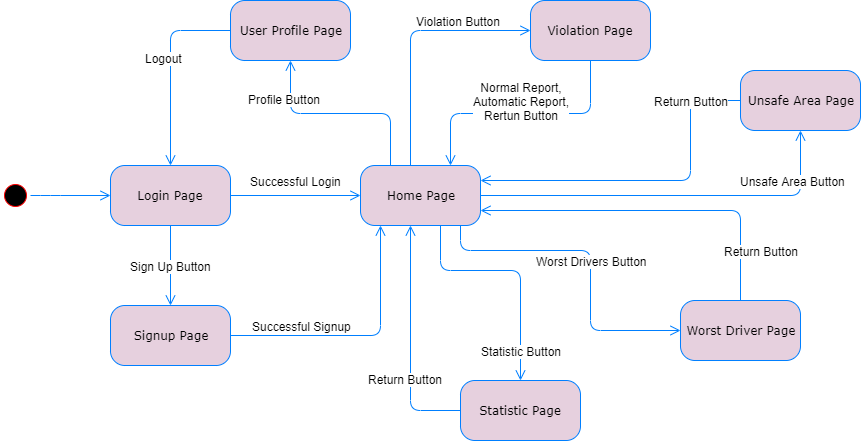
\includegraphics[width=1.2\textwidth]{images/uxDiagram}}
\caption{The initial UX diagram} 
\label{fig:basicux} 
\end{figure} 
\end{center}
\subsection{Mockups of the User Interface}
\begin{figure}
	\begin{flushleft}
		\textbf{Login Page}:\\
		Since logging into SafeStreets is mandatory, this is the first page that the user will face when the app does not recognizes him. Of course, cookies or sessions could avoid to force the user to login every time.
	\end{flushleft}
	\centering
	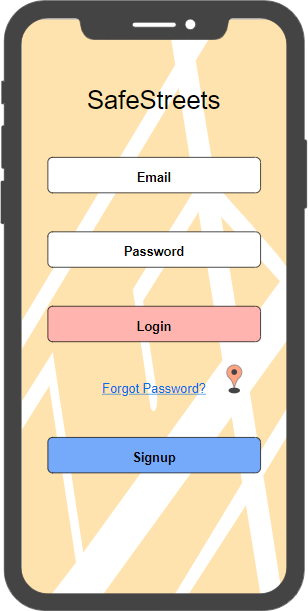
\includegraphics[width=0.6\linewidth]{../RASD/images/mockups/login}
	\caption{SafeStreets Login page.}
\label{fig:login}
\end{figure}
\clearpage
\begin{figure}
	\begin{flushleft}
		\textbf{SignUp Page}:\\
		Since logging into SafeStreets is mandatory, if the user does not have an account he needs to make one. Every field except the photo should be mandatory.
	\end{flushleft}
	\centering
	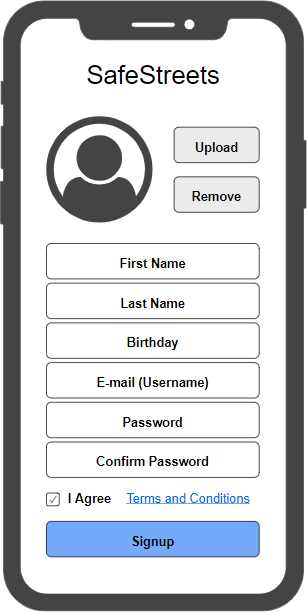
\includegraphics[width=0.6\linewidth]{../RASD/images/mockups/signup}
	\caption{SafeStreets SignUp page.}
	\label{fig:signup}
\end{figure}
\clearpage
\begin{figure}
	\begin{flushleft}
		\textbf{Home Page}:\\
		When the user logs into SafeStreets successfully, an home page should be provided with the options for the user to use every functionality of the application.
	\end{flushleft}
	\centering
	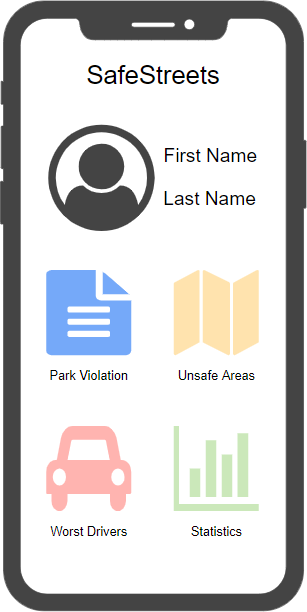
\includegraphics[width=0.6\linewidth]{../RASD/images/mockups/homePage}
	\caption{SafeStreets Home page.}
	\label{fig:home}
\end{figure}
\clearpage
\begin{figure}
	\begin{flushleft}
		\textbf{Violation Page}:\\
		If the user wants to send to the officers a parking violation of some sorts a form to be filled is provided. The user can either send a report that will generate an automatic ticket or that will need to be checked by the officers.
	\end{flushleft}
	\centering
	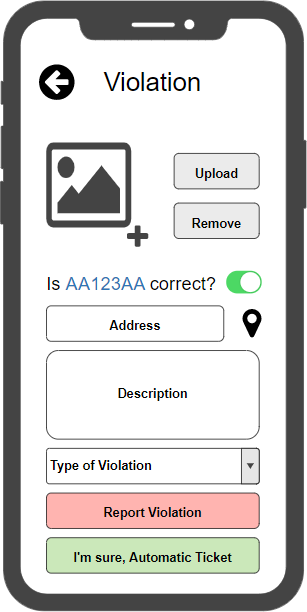
\includegraphics[width=0.6\linewidth]{../RASD/images/mockups/violation}
	\caption{SafeStreets Violation page.}
	\label{fig:violation}
\end{figure}
\clearpage
\begin{figure}
	\begin{flushleft}
		\textbf{Unsafe Areas Page}:\\
		If the user wants to see which areas are the most subject to violations, an interface to search among all areas should be implemented.
	\end{flushleft}
	\centering
	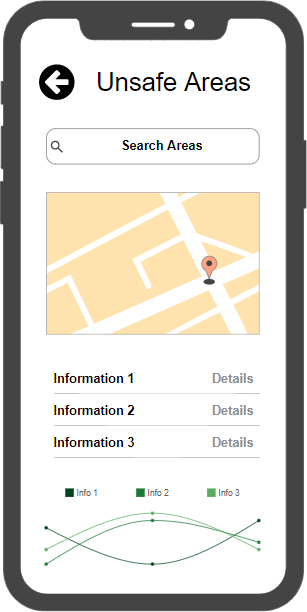
\includegraphics[width=0.6\linewidth]{../RASD/images/mockups/areas}
	\caption{SafeStreets Unsafe Areas page.}
	\label{fig:areas}
\end{figure}
\clearpage
\begin{figure}
	\begin{flushleft}
		\textbf{Worst Drivers Page}:\\
		If the user wants to see which vehicles tends to not follow the city rules, an interface that shows this needs to be present in the application.
	\end{flushleft}
	\centering
	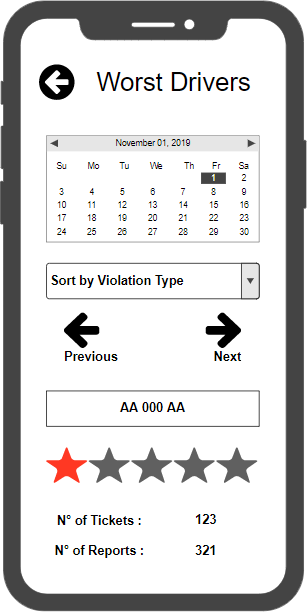
\includegraphics[width=0.6\linewidth]{../RASD/images/mockups/vehicles}
	\caption{SafeStreets Worst Drivers page.}
	\label{fig:vehicles}
\end{figure}
\clearpage
\begin{figure}
	\begin{flushleft}
		\textbf{Statistics Page}:\\
		A complete page that exhibits all of SafeStreets data in a complete and detailed manner, that also enlightens SafeStreets effectiveness. 
	\end{flushleft}
	\centering
	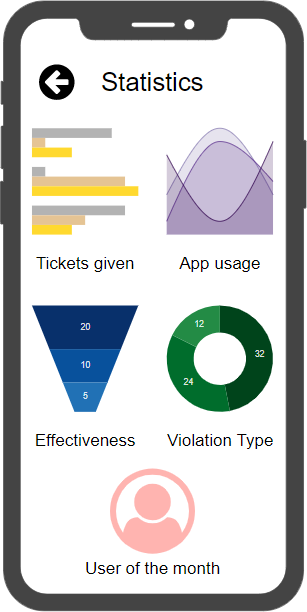
\includegraphics[width=0.6\linewidth]{../RASD/images/mockups/statistics}
	\caption{SafeStreets Statistics page.}
	\label{fig:statistics}
\end{figure}
\clearpage
\begin{figure}
	\begin{flushleft}
		\textbf{User Profile Page}:\\
		If the user wants to change its profile picture or his password, if he wants to check his reports or to logout, he should be able to do all these things. 
	\end{flushleft}
	\centering
	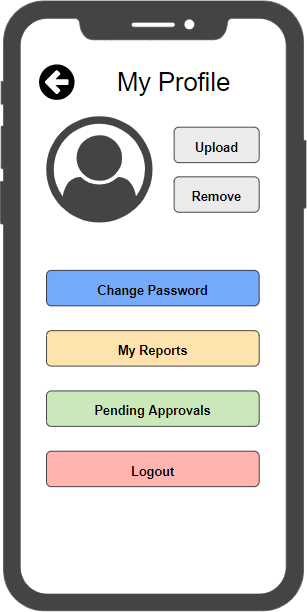
\includegraphics[width=0.6\linewidth]{../RASD/images/mockups/profile}
	\caption{SafeStreets User Profile page.}
	\label{fig:profile}
\end{figure}
\clearpage
\clearpage
\section{Requirements Traceability}
In order to have a simplified and schematic view over the designed components that are going to satisfy the requirements and provide the functionalities which were identified in the RASD we define a formal mapping that explicitely correlates the Goals and functions with one or more Components that should be able to achieve the goal and create the functionality.



\begin{table}[htp]
\begin{center}
\begin{tabular}{|p{5cm}|p{5cm}|p{5cm}|}
\hline
Goal&Functions&Components\\
\hline
\textbf{[G1]:}Allowing users to notify officers when particular parking violations occur.&
\textbf{[F1]:}Notification of Violations&
\textbf{[M2:]}\hyperlink{watson}{IBM Watson Visual Recognition}\newline\textbf{[M4:]}\hyperlink{cloudObjectStorage}{IBM Cloud Object Storage}\\
\hline
\textbf{[G2]:}Permitting both users and officers to learn which are the most unsafe areas in their jurisdiction.&
\textbf{[F2]:}Data Mining&
\textbf{[M3:]}\hyperlink{discovery}{IBM Discovery}\newline\textbf{[M6:]}\hyperlink{postgres}{IBM Cloud Databases for PostgreSQL}\\
\hline
\textbf{[G3]:}Suggesting possible interventions to potentially unsafe areas in the city.&
\textbf{[F3]:}Request for interventions&
\textbf{[M3:]}\hyperlink{discovery}{IBM Discovery}\newline\textbf{[M5:]}\hyperlink{cloudant}{IBM Cloudant}\\
\hline
\textbf{[G4]:}Allowing the authorities to generate automatic parking violation tickets from users’ reports.&
\textbf{[F4]:}Automatic Tickets&
\textbf{[M2:]}\hyperlink{watson}{IBM Watson Visual Recognition}\newline\textbf{[M3:]}\hyperlink{discovery}{IBM Discovery}\\
\hline
\textbf{[G5]:}Permitting both users and officers to learn which vehicles commit the most violations.&
\textbf{[F2]:}Data Mining\newline\textbf{[F5]:}Statistics&
\textbf{[M3:]}\hyperlink{discovery}{IBM Discovery}\newline\textbf{[M6:]}\hyperlink{postgres}{IBM Cloud Databases for PostgreSQL}\\
\hline
\textbf{[G6]:}Permitting customers to apprehend the possible effectiveness of these mechanisms.&
\textbf{[F2]:}Data Mining\newline\textbf{[F5]:}Statistics&
\textbf{[M3:]}\hyperlink{discovery}{IBM Discovery}\newline\textbf{[M6:]}\hyperlink{postgres}{IBM Cloud Databases for PostgreSQL}\\
\hline
\textbf{[G7]:}Allowing both users and officers to learn the analytics of the tickets given in their city.
&
\textbf{[F2]:}Data Mining\newline\textbf{[F5]:}Statistics&
\textbf{[M3:]}\hyperlink{discovery}{IBM Discovery}\newline\textbf{[M6:]}\hyperlink{postgres}{IBM Cloud Databases for PostgreSQL}\\
\hline
-&\textbf{[F0]:}User data management&\textbf{[M1:]}\hyperlink{appid}{IBM App ID}\\
\hline
\end{tabular}
\end{center}
\caption{Requirements Traceability} 

\end{table}
\clearpage
\section{Implementation, Integration and Test Plan}
\subsection{Implementation Order}
Here we explain how a possible good order of implementation of sub-components might help us to fulfill and build the application. Its achievement implies the following steps:
\begin{itemize}
	\item The very first thing to be implemented is the SafeStreets link with the municipality, implemented in form of encrypted HTTP APIs. The correct and secure definition of this link is something that the entire SafeStreets architecture relies on.
	\item At the second stage, we plan to create and configure all the server components/microservices (since they are those which will be queried by the client application afterwards).
	\\Every microservice component, will be implemented following the goals and functionalities described in this documents and in the SafeStreets RASD. The order of the implementation of each microservice is not relevant, but only the development of one microservice at a time will be allowed.
	Basically, our implementation order ranges from creating a user pool (IBM App ID) for data synchronization and authentication to setting up the cloud storage (IBM Cloud Object Storage and IBM Cloudant) for archiving data. 
	\item Then, when all microservice are implemented, we will focus on the creation of the client application such as the mobile app and the dashboard for the municipality.
\end{itemize}

As said, in our architecture, every microservice needs to be developed one small functionality at a time, and should be as atomic as possible. Once a microservice is ready, it will be tested on its own, in order to have a more efficient way of testing the application.

\subsection{Macrocomponents to be integrated}
\subsection{Integration Testing Strategy}
The first integration testing strategy that we'll use to test our application during its development, is the \textbf{Thread approach}. In particular, the \textbf{Bottom-up strategy} will be used to test and integrate modules within every thread. At first, only single portions of the modules (the ones that don't need any stubs) will be integrated and tested.
\\Small drivers needs to be created in order to give inputs to the portion of each module until a single feature is completed, then others threads will replicate the same procedure with the goal of reaching the completeness of the whole application.
\\Using a global strategy like this one will allow to have an application that works in the early stages of the implementation; this could permit to anticipate some testing and could minimize the costs of repair in the eventuality of an error.
\\Having said that, we will perform a second integration test when each module is fully implemented
\\In this new tests, we will impersonate a user who is actually using our application and who tries to get a result in response to a certain action.
\\This kind of test verifies not only the correct behavior of every single element, but also ensure the correct relationships with the other components of the application, listed in the above subsection.
\\The integration test that we will set up will use a real browser or application in order to perform, on the pages of the application, a certain number of actions in a programmatic way (such as the submission of a violation), to then verify a specific output at the end of the test. Following the example of the violation submission, the user will expect a successful message.
\\Although the integration test is undoubtedly the most complete and reliable, since it runs the entire stack during its execution, it is also the slowest, especially for the functionality that to be tested requires interaction with Computer Vision or Data Mining.
\\In our case, we would have needed to collect thousand of test results, but integrating the component with the thread approach while developing allow ou to proceed with fewer integration tests and then lower the execution times.


\clearpage
\section{Softwares Used, Effort Spent and History}
\begin{flushleft}
\textbf{Software Used}
\end{flushleft}
\begin{table}[htp]
	\centering
		\begin{tabular}{|c|c|}
			\hline
			Task&Software Used\\
			\hline
			Edit and compile LATEX code&TeXstudio and VisualStudioCode\\
			\hline
			UML modelling&PlantUML\\
			\hline
			Images and charts&draw.io\\
			\hline
			Run and compile Alloy&Alloy 4.2\\
			\hline
			Mockup&Moqups\\
			\hline
		\end{tabular}
	\caption{Softwares used} 
\end{table}
\begin{flushleft}
\textbf{Effort Spent}
\end{flushleft}
\begin{table}[htp]
	\centering
		\begin{tabular}{|c|c|}
			\hline
			Student&Hours spent\\
			\hline
			Andrea Furlan&-\\
			\hline
			Cosimo Russo&-\\
			\hline
			Giorgio Ughini&-\\
			\hline
		\end{tabular}
	\caption{Effort spent} 
\end{table}


\end{document}

